% define \title (only used by writelatex.com)
%\title{CSEC-793 Project Report_Blank}
%%%%%%%%%%%%%%%%%%%%%%%%%%%%%%%%%%%%%%%%%%%%%%%%%%%%%%%%%%%%%%%%%%%%%%
% LaTeX Template: Project Titlepage
%
% Source: http://www.howtotex.com
% Date: April 2011
% [p]
% This is a title page template which be used for articles & reports.
% 
% Feel free to distribute this example, but please keep the referral
% to howtotex.com
% 
%%%%%%%%%%%%%%%%%%%%%%%%%%%%%%%%%%%%%%%%%%%%%%%%%%%%%%%%%%%%%%%%%%%%%%
% How to use writeLaTeX: 
%
% You edit the source code here on the left, and the preview on the
% right shows you the result within a few seconds.
%
% Bookmark this page and share the URL with your co-authors. They can
% edit at the same time!
%
% You can upload figures, bibliographies, custom classes and
% styles using the files menu.
%
% If you're new to LaTeX, the wikibook is a great place to start:
% http://en.wikibooks.org/wiki/LaTeX
%
%%%%%%%%%%%%%%%%%%%%%%%%%%%%%%%%%%%%%%%%%%%%%%%%%%%%%%%%%%%%%%%%%%%%%%
%
% --------------------------------------------------------------------
% Preamble
% --------------------------------------------------------------------
\documentclass[ fontsize=11pt,twoside]{scrartcl}	% KOMA

\usepackage[letterpaper,pdftex]{geometry}	% A4paper margins
\setlength{\oddsidemargin}{5mm}			% Remove 'twosided' indentation
\setlength{\evensidemargin}{5mm}

\usepackage[english]{babel}
\usepackage[protrusion=true,expansion=true]{microtype}	
\usepackage{amsmath,amsfonts,amsthm,amssymb}
\usepackage{graphicx}
\usepackage{pseudocode}

\usepackage[latin1]{inputenc}
\usepackage{tikz}
\usetikzlibrary{shapes,arrows}


% --------------------------------------------------------------------
% Definitions (do not change this)
% --------------------------------------------------------------------
\newcommand{\HRule}[1]{\rule{\linewidth}{#1}} 	% Horizontal rule

\makeatletter							% Title
\def\printtitle{%	
    {\centering \@title\par}}
\makeatother									

\makeatletter							% Author
\def\printauthor{%					
    {\centering \Large \@author}}				
\makeatother							

% --------------------------------------------------------------------
% Metadata (Change this)
% --------------------------------------------------------------------
\title{	\Large \textsc{ ECE 657A- Data and Knowledge Modeling and Analysis \\ } 
		 	\\[1.0cm]								% 2cm spacing
			\HRule{2pt} \\					    	% Upper rule
			\LARGE \textbf{\uppercase{Assignment 2 Report}}	% Title
			\HRule{2pt} \\ [0.5cm]		% Lower rule + 0.5cm spacing
			\Large \today			    % Todays date
		}
        
 \author{
		Adam Kulas -\texttt{UW ID: 20302000}\\	
        Richard Ozara -\texttt{UW ID: 20801583 } \\
        Ammar Ahmed -\texttt{UW ID: 20734898}\\
		Department of Electrical and Computer Engineering\\	
		University of Waterloo \\ 
}



\begin{document}
% ------------------------------------------------------------------------------
% Maketitle
% ------------------------------------------------------------------------------
\thispagestyle{empty}		% Remove page numbering on this page
\printtitle 				% Print the title data as defined above
  	\vfill
\printauthor				% Print the author data as defined above
\newpage

% ------------------------------------------------------------------------------
% Begin document
% ------------------------------------------------------------------------------
\setcounter{page}{1}		% Set page numbering to begin on this page

%%%%%%%%%%%%%%%
%														%
% 			Main Contents                               %
%														%
%%%%%%%%%%%%%%%

\section{Question I: Revisiting HW4 Bank Classification with New Tools (for dataset A)}
\subsection{Data preprocessing}
For this part of the assignment, the dataset had to be analyzed first as part of the preprocessing step to get the structure ,detect issues such as missing values and outliers. The bank marketing data(bank-additional.csv) has 4119 observations and 21 features.There was found to be 1230 unknowns in the categorical features of the dataset. Features that had unknowns were checked and there was found to be six features: job,marital,education,default,housing,loan that had unknowns( 0.96 ,0.3 ,4.1,  19.5, 2.6)\% respectively.Removing rows with missing values can be too limiting on some predictive modeling problems. The proportion of the unknown's is sparse, the mode of the categorical features was used to replace the unknown's. Also, the "duration" feature was dropped since this attribute highly affects the output target (e.g., if duration=0 then y='no').
The categorical predictor variables  were converted  to numerical using get\_dummies ,appending the structure to 47 features (4119,47).
Outliers were found by first finding the standard deviation of each feature and then using each standard deviation to find values in that specific feature that vary by more than 3 standard deviations. 

\subsection{Dividing data into training and testing}
For dividing the data-set(4119 samples), 80\% was used for training and 20\% for testing. The reason for this split is because of the data imbalance as we have  3,668 samples labeled as no as compared to 451 labeled as yes. By using 80\% of the data for training the model, we are providing more information for the model to learn about the yes which improves the prediction for this label. %The 80-20 split ensures all cases is accounted for in the training phase and our algorithm is generalizing and not memorizing. 


\subsection{Applying classification}
%Figure~\ref{fig:fig1} shows the comparison between histogram plots of feature 9 and 24 before and after normalization. 

Decision Tree (DT):\\ The Depth of the tree was chosen as 3 for which the model performed more accurately without over-fitting. We first plotted the area under curve score (AUC score) against the tree depth (figure 1 below).
\begin{figure}[!ht]
 \centering
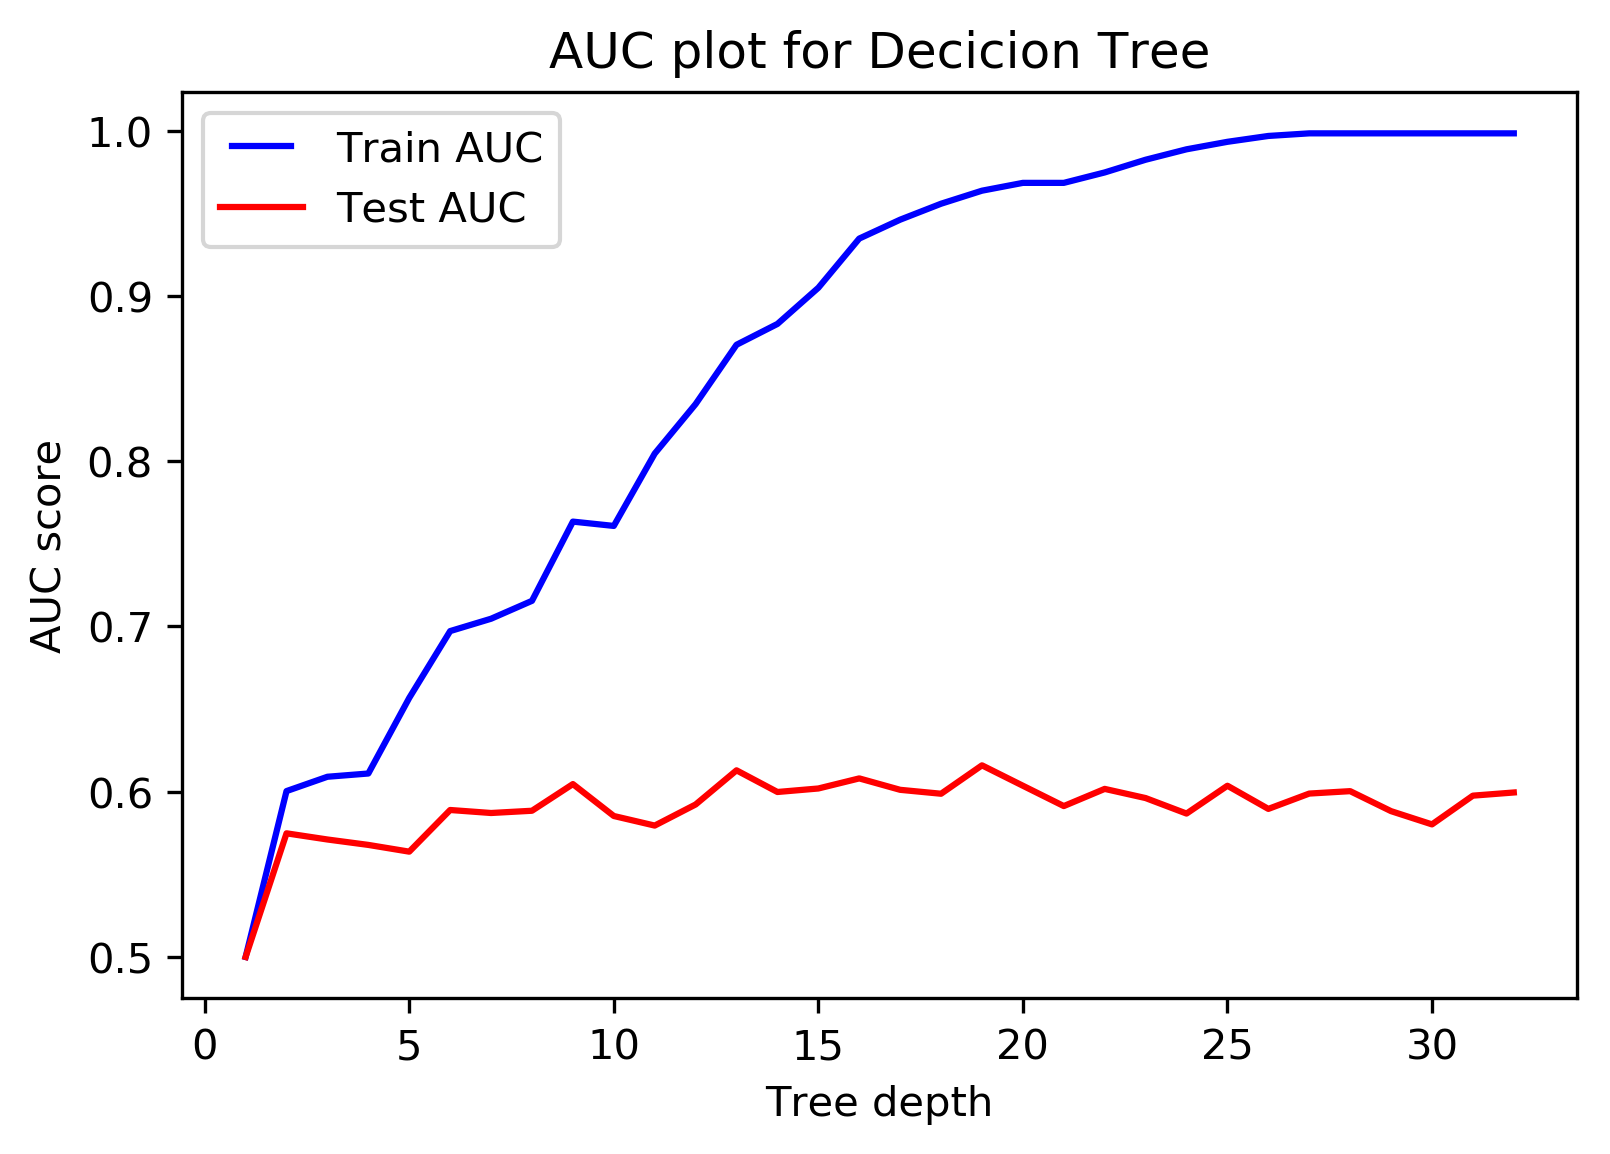
\includegraphics[width=6.1in]{assignment2/1-3-DecisionTree_AUC.png}
\caption{\label{fig:fig1}AUC score curve against tree depth}
\end{figure}
As it can be seen from the curve, the deeper the tree the higher the train AUC score but the test AUC score wont change a lot after tree depth of 3. This means that we get an overfitting case as our model will have a high AUC score (predicts the train data perfectly) for deeper tree depth but will fail to generalize and predict the test data. For this reason the tree depth was chose to be 3 for our model.
If the depth of tree was not specified, by default, scikit-learn will keep expanding the nodes until all the leaves contain less than min\_samples\_split samples and as we saw in the graph below, the higher value of maximum depth causes over-fitting, and a lower value causes under-fitting\cite{ref_url1}.


ID3, or Iternative Dichotomizer, was the first of three Decision Tree implementations developed by Ross Quinlan
It builds a decision tree for the given data in a top-down fashion, starting from a set of objects and a specification of properties Resources and Information. each node of the tree, one property is tested based on maximizing information gain and minimizing entropy, and the results are used to split the object set. This process is recursively done until the set in a given sub-tree is homogeneous (i.e. it contains objects belonging to the same category). The ID3 algorithm uses a greedy search. It selects a test using the information gain criterion, and then never explores the possibility of alternate choices.

CART stands for Classification and Regression Trees. It is characterized by the fact that it constructs binary trees, namely each internal node has exactly two outgoing edges. The splits are selected using the twoing criteria and the obtained tree is pruned by cost–complexity Pruning. CART can handle both numeric and categorical variables and it can easily handle outliers.
\\

Random Forests (RF): \\
The random forests classifier was built using the scikit-learn. The two main parameters that were considered here are the n\_estimator and tree depth. The n\_estimator simply represnts the number of trees in the model and tree depth is the depth of those tree. Similar to the approach described in the decision tree, AUC score was plotted against n\_estimator and tree depth to avoid any over-fitting cases. Figure~\ref{fig:fig2} shows the AUC scores for n\_estimator and figure~\ref{fig:fig3} shows the AUC scores for tree depth. 
\begin{figure}[!ht]
 \centering
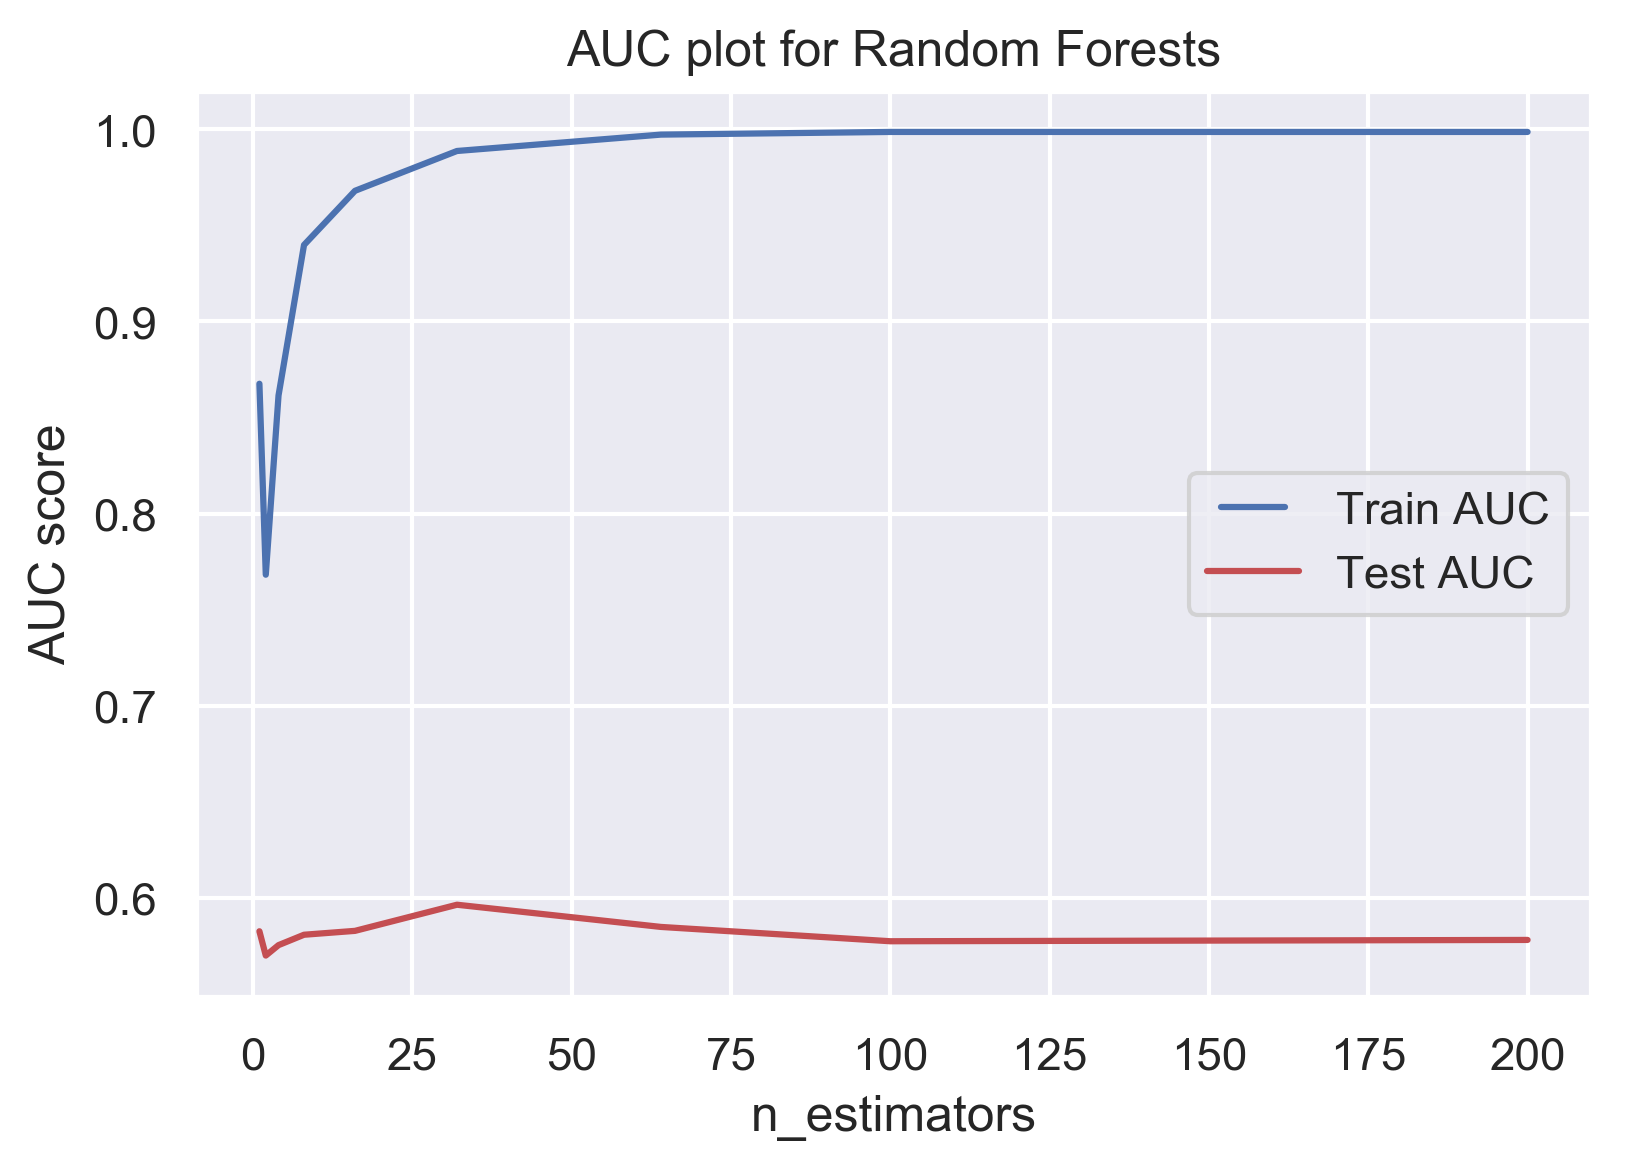
\includegraphics[width=6.1in]{assignment2/1-3-RandomForests_AUC(n_estimators).png}
\caption{\label{fig:fig2}AUC score curve against n\_estimators}
\end{figure}

\begin{figure}[!ht]
 \centering
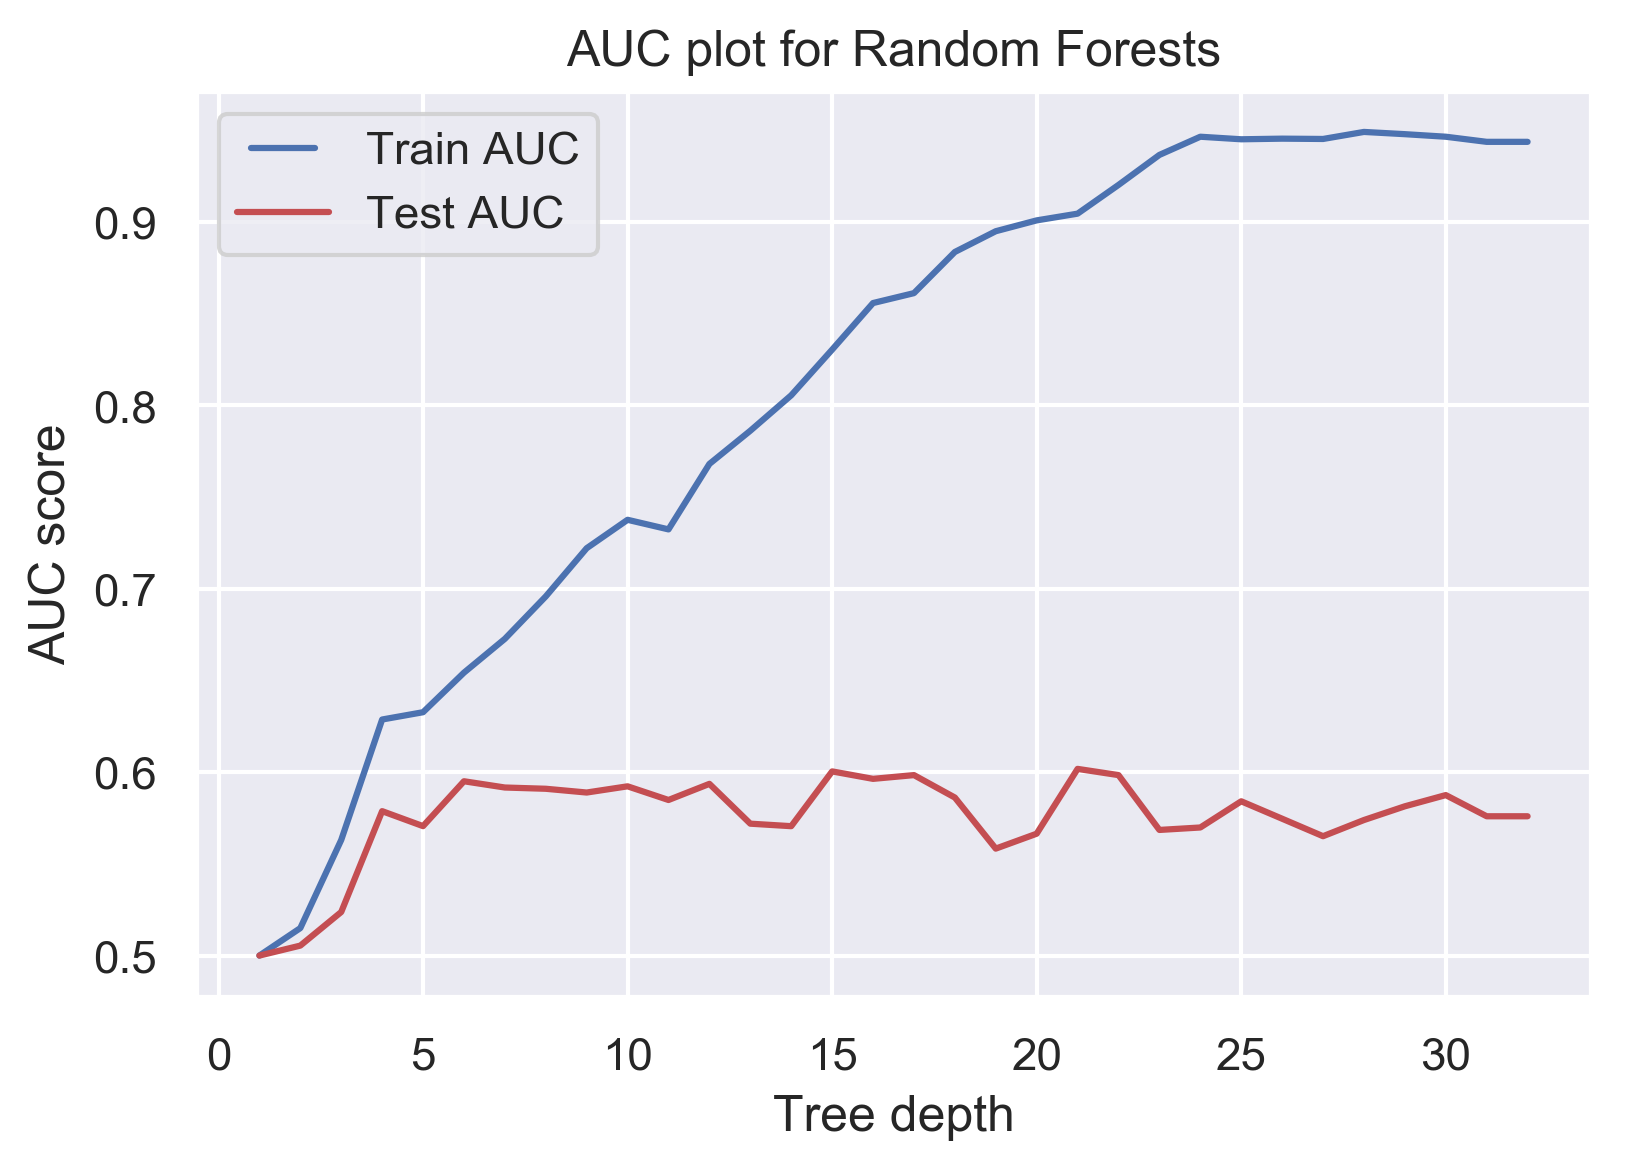
\includegraphics[width=6.1in]{assignment2/1-3-RandomForests_AUC(TreeDepth).png}
\caption{\label{fig:fig3}AUC score curve against tree depth}
\end{figure}

\\

Neural Network (NN): \\
Neural netwrok is made up of three main layers: input, hidden, and output layers. In our case, the input layer is made up of 46 layers (number of input features) and the output layer has a single node (outputs either 1 or 0). The way the neural network model works is that it receives an inputs and multiply them by some weight which is then passed to an activation function to predict an output. Then the output is compared with y\_test label in which the weights will be adjusted accordingly. The process repeated until the maximum number of iterations reached. For building our model, we used gridsearch built-in function which returns the best hyper-parameters from the parameter space list provided. The hyper-parameters that were tested are:\\
1- hidden layer sizes : [(32,32), (20,20), (47,47)] \\
2- activation function: ['tanh', 'relu'] \\
3- solver: ['sgd', 'adam','lbfgs'] \\
4- alpha: [0.0001, 0.05] \\
then the gridsearch returned the parameters that best performed. However, one thing to note is that even though there is no rule of thumb for choosing the number of neurons in the hidden layers, it should not exceed the number of input layers (46 in this case) to avoid over-fitting problems. 
The best parameters were found to be as follow: activation=tanh, alpha=0.0001, hidden layers = (32, 32), and solver = Stochastic Gradient Descent (SGD). 

\\
\subsection{Create a few plots of your model on the test data, two of the data dimensions at a time,indicating the predicted elements of each class using different colors or shapes. You may need to try plotting various pairs of dimensions to see which provide some interesting result. Be sure to label your axis and legend. Why is separation better on some plots than others}

\\



\subsection{Produce a table with the true/false positive/negative metrics as well as accuracy's. Compare the values using bar charts}

Figure~\ref{fig:fig4} shows the comparison between true/false positive/negative metrics as well as accuracies
\begin{figure}[!ht]
 \centering
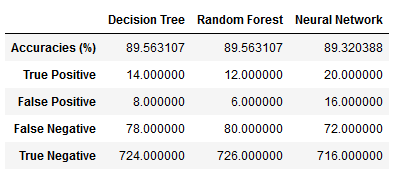
\includegraphics[width=6.1in]{assignment2/1-5_table.png}
\caption{\label{fig:fig4}table of metrics/accuracies and algorithms}
\end{figure}

Figure~\ref{fig:fig5} shows the comparison between true/false positive/negative metrics as well as accuracies
\begin{figure}[!ht]
 \centering
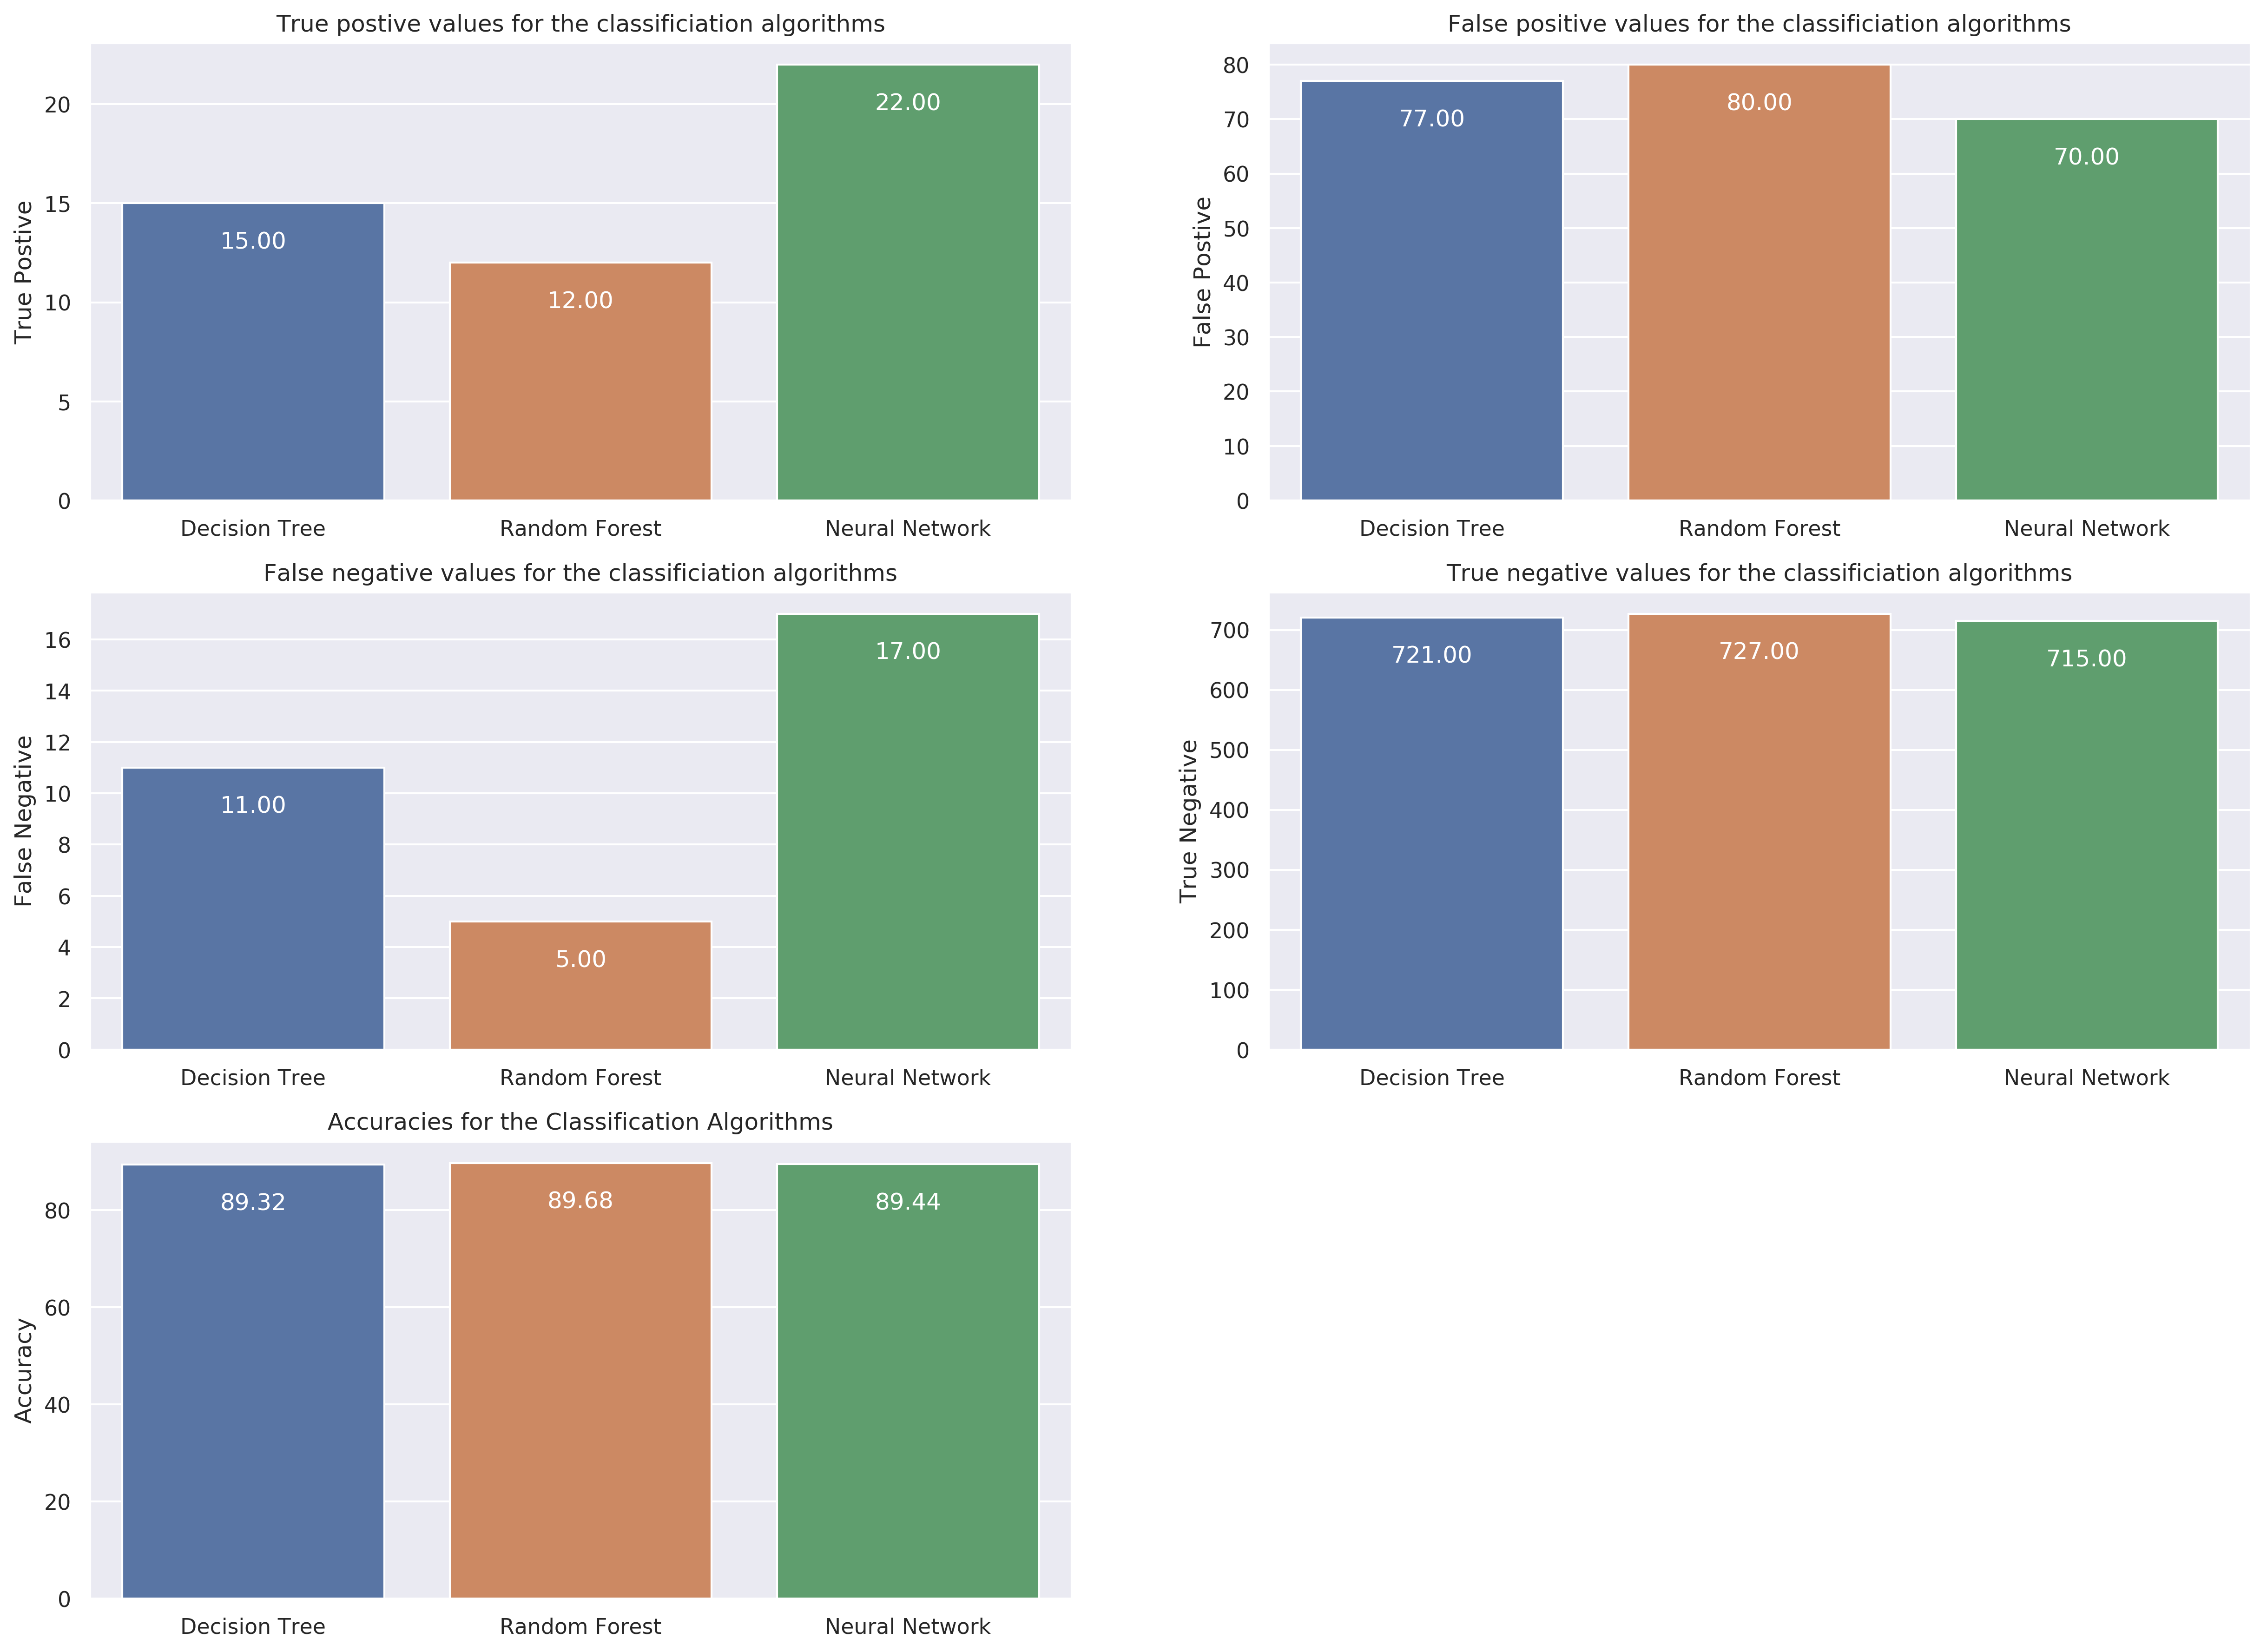
\includegraphics[width=6.1in]{assignment2/80-20_barcharts_algorithms.png}
\caption{\label{fig:fig5}bar charts of metrics/accuracies and algorithms}
\end{figure}

\\

\subsection{Provide a short explanation of the results you have shown and what it means. Which classification method performed better? Why? Contrast performance with classification from the previous homework and comment on the difference, if any}


\\

\subsection{ Fun/Bonus: attempt at least one method to tackle the discrepancy in the size of the classes (imbalanced data)}
 I think to tackle the issue of imbalanced data,precision should be used when analyzing best threshold for each algorithm using ROC/AUC .As we know , AUC uses TPR(True positive rate) on Y axis and FPR(False positive rate ) on X axis. So replacing the FPR with precision on the X axis of the AUC graph might be the way to go.
 Precision=(TP/TP +FP) FPR= (FP/TN+FP)
 Since there were lots of samples that were Negatives(No's) relative to the number of Positives(Yes's) samples, then precision might be more useful than false positive rate . This is because precision does not include the number of True Negatives in its calculation, and is not affected by imbalance.




\section{Question 2:Parameter Selection and Classification (for dataset B)}
\subsection{Data preprocessing}
Z-score normalization was used for normalizing data instead of the min-max normalization. The Z-Score normalization is a standardization and re-scaling the range of the data in which the mean is centered on zero and it has a unit variance. This means that z-score will still preserve the range of the data (maximum and minimum) as min-max normalization but also will provide the standard deviation and variance of the distribution. This is helpful when it comes for dealing with data flowing in real time as we can easily normalize data coming in using the mean and variance, however, if we used min-max normalization then we might run into an issue where the data coming in is larger than the max the we trained model. This is an advantage that we get by choosing the z-score over the min-max. \\
We split the test and training set randomly in order to evaluate the performance of the models (Classifiers). \\
For this dataset, the distribution of the labels is almost the same. We have 1137 samples labeled as 1 and 1063 samples labeled as -1.


\\
\subsection{Parameter selection:}
\subsubsection{Parameter selection for k-NN}

A k-NN classifier was employed to predict the labels of the data in data set B based on the input of the 56 features. The main hyper parameter of the k-NN model is the number of neighbours, "k". A set of possible values for the hyper parameter were tested and validated using 5 fold cross validation. Each fold represents a slice of the data and one fold at a time is used as the validation set to verify the performance of the model. This model was not validated directly on the test set because 5 fold cross validation intentionally using one of the folds as a test set. In the case of 5 fold the resulting test train split is effectively 80/20. The test set can then be used to compared different models with equal fairness knowing that none of the data would bleed through during the cross validation step.

For each value of K the cross validated accuracy score was returned as the key performance metric. Figure~\ref{fig:knntuning} shows the plot of the accuracy vs the value  of the parameter "k". We see that the model performed best when the value of "k" was set to 15.

\clearpage{}
\begin{figure}[!ht]
 \centering
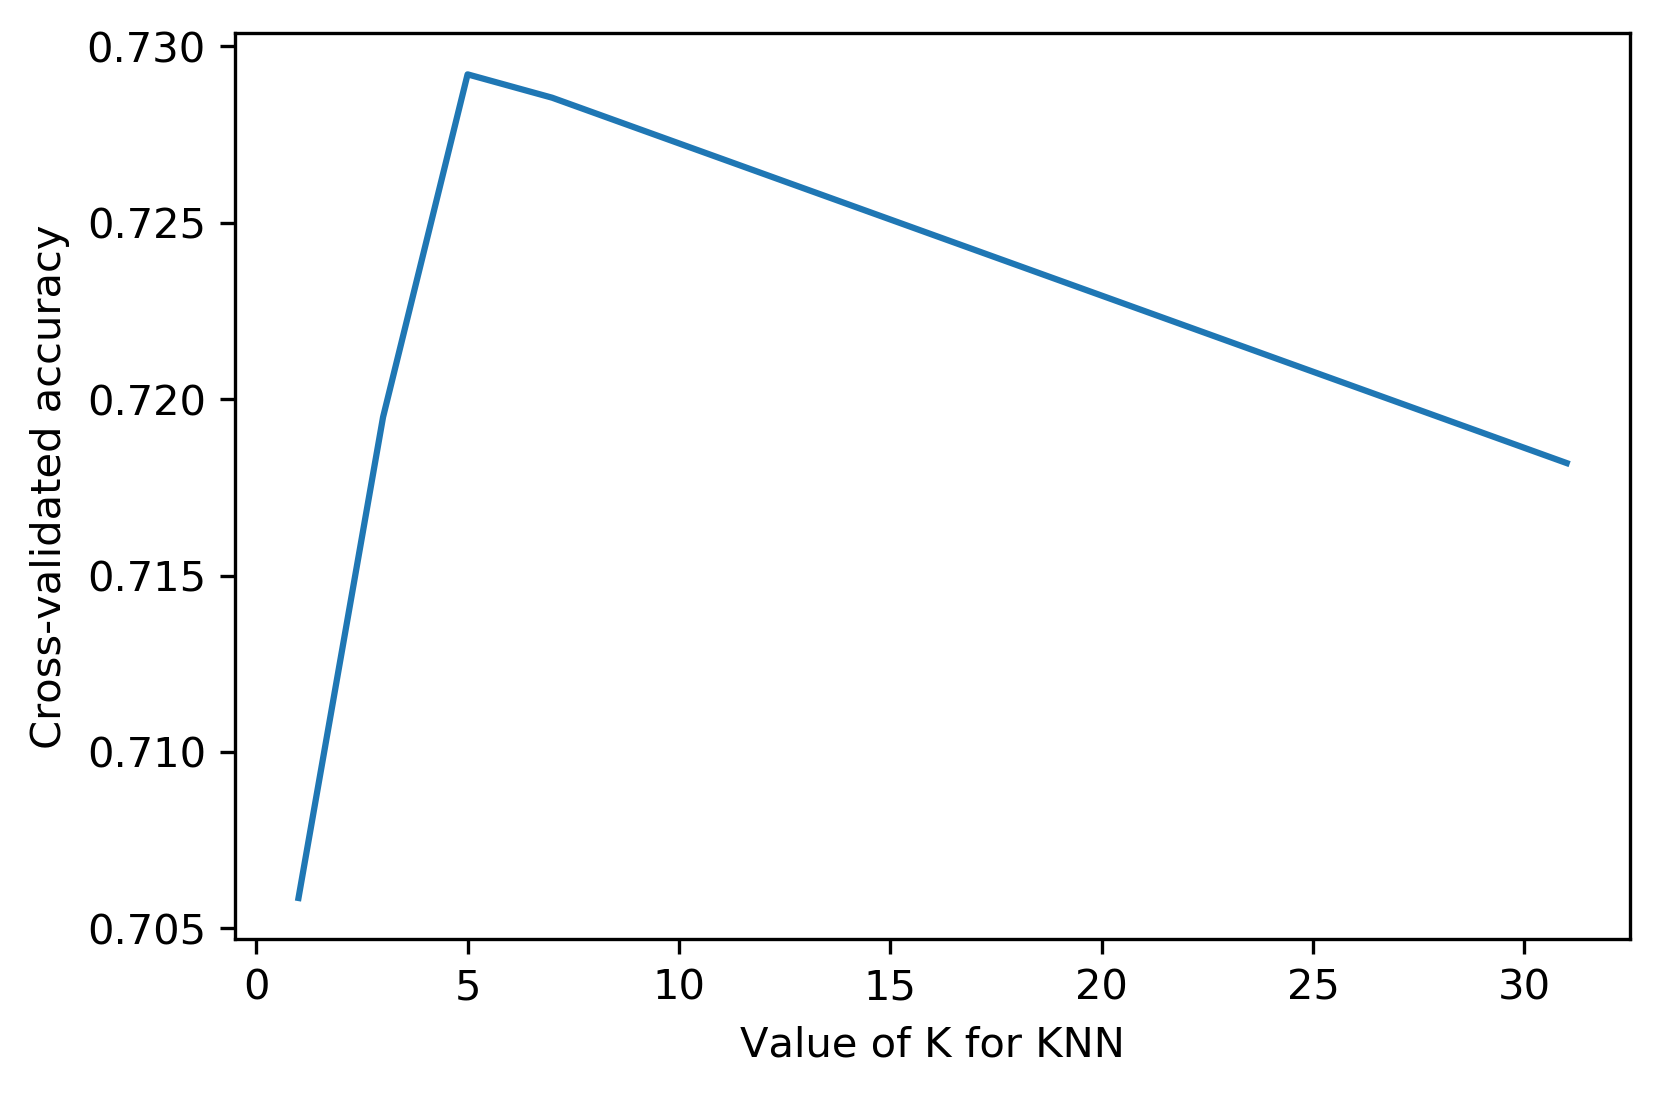
\includegraphics[width=6.1in]{assignment2/2-2-a-kNN.png}
\caption{\label{fig:knntuning} Relationship between accuracy and the parameter k }
\end{figure}



\subsubsection{Parameter selection for SVM}

A support vector machine model was created to predict labels of the given data set. There were two hyper parameters that need to be determined for the SVM model, "C" and "gamma". In order to determine the optimal values a grid search was done over the parameter space with the given set of values. The scoring metric used for each combination of parameters was "roc_auc". The result of the hyper parameter tuning was a value of 0.01 for gamma and 10 for C.

The model was then trained on the training data using the hyper parameters found during the cross validation grid search. Figure~\ref{fig:svmtuning} shows the plot of AUCROC for the tuned and trained SVM model. The AUC of the model is 0.97.


\begin{figure}[!ht]
 \centering
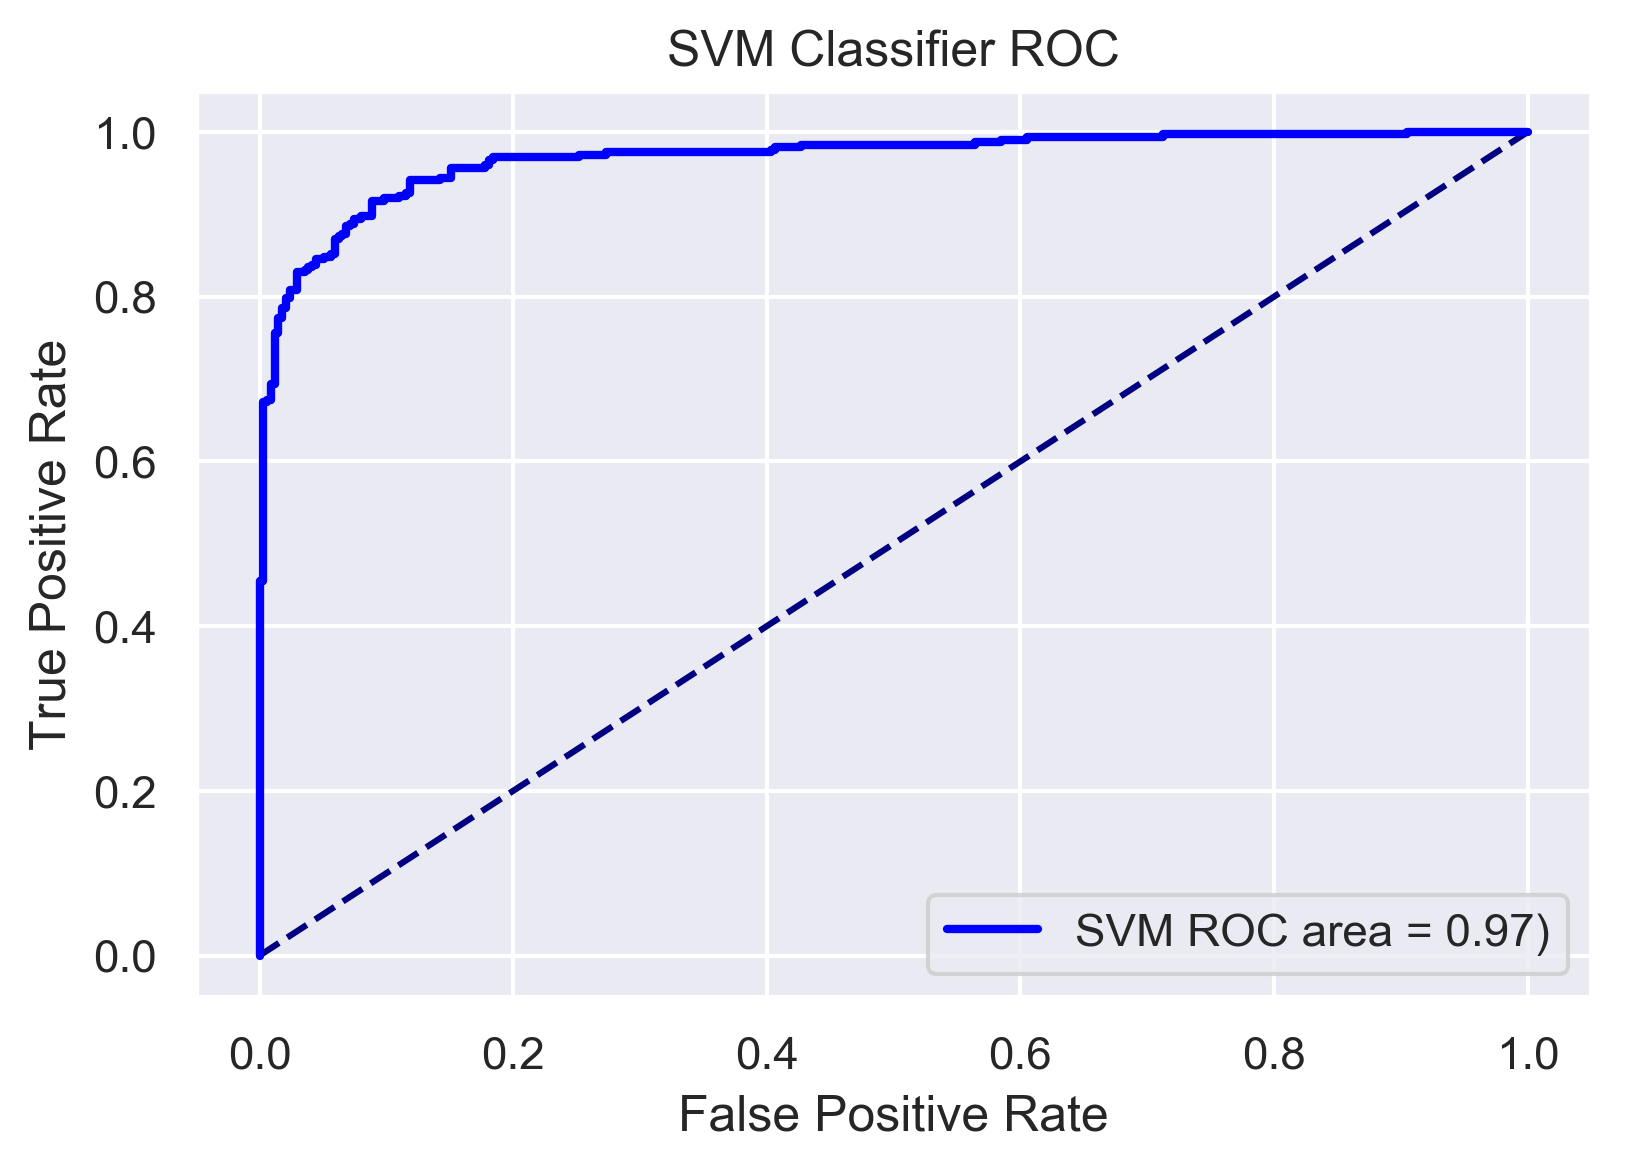
\includegraphics[width=6.1in]{assignment2/2-2-b-svm.png}
\caption{\label{fig:svmtuning} SVM area under curve receiver operator characteristic}
\end{figure}


\subsection{Training six classifiers}

\subsubsection{Classify the test set using k-NN, SVM, Random Forests and Neural Networks. Use the chosen parameters from the parameter selection process in question 2 for k-NN and SVM. For the next two classifiers use the default setups listed at the end for Random Forests and Neural Networks}


The performance for the four models (KNN, SVM, Random Forest and Neural Network) was calculated using the sklearn library function "classification\_report". We can see the results of the classification in Figure~\ref{fig:resultsknnsvm} and Figure~\ref{fig:resulstsrfnn} below. From the results we can see that the KNN model performed the worst with an average F1 score of 0.75. The SVM model and Neural Network with default parameters performed similarly with and average f1 score of 0.91 and 0.90 respectively. Finally the random forest model out performed the other models with an average f1 score of 0.95.

It is important to mention that there are multiple metrics that can be used to evaluate the performance of a model on a binary classification problem. Depending on the data provided and the use case of the model some outcomes may be more desired that others. For example the true positive rate may be more important for a bank to determine default likelihood because of the impact to their business if a false negative is provided. Knowing this it may be more important to value recall over precision or vice-versa. The f1-score does a decent job of blending the performance of both scenarios and is therefore used in this report as the general metric to evaluate performance between these models.

Overall there is not much variation between the various scoring metrics. This is most likely due to the fact that the data set provided is fairly balanced. The count of the true labels and false labels is quite similar. If the data was imbalanced techniques could have been used to reduce the impact to the models where labels are biased to the majority class. This problem may have been an issue for the classifiers found in part 1 as there was a large imbalance between the majority and minority classes.

% \clearpage{}
\begin{figure}[!ht]
 \centering
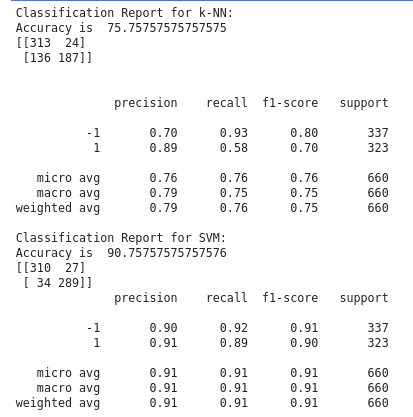
\includegraphics[height=3.5in]{assignment2/2-3-a1.png}
\caption{\label{fig:resultsknnsvm} Performance Result for KNN and SVM models using parameters from section 2.2}
\end{figure}
\clearpage{}
\begin{figure}[!ht]
 \centering
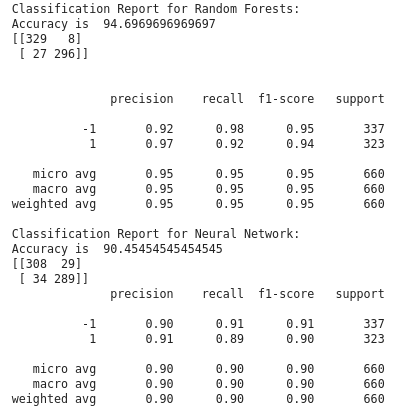
\includegraphics[height=3.5in]{assignment2/2-3-a2.png}
\caption{\label{fig:resulstsrfnn} Performance Result for Random Forest and Neural Network models using default parameters}
\end{figure}


\subsubsection{For the fifth and sixth classifiers, you should explore the parameters of the Random Forests and Neural Network models to devise your own classifier instance that does better than the other methods. For example, you could consider a deeper neural network with multiple layers, use different optimization/solver algorithms, you could modify the Random Forests using different parameter settings for depth and number of trees or enable boosting. Play around with options and choose a setting for RFs and NNs that performs better}

Our first goal is to increase the performance of the random forest model in predicting the test subset of the provided data set. Our approach is to use linear search over two important hyper parameters of the random forest model, "n\_estimators" and "treedepth". Figure~\ref{fig:rfnest} below shows the plot of AUC for both the train and test data. We can see from the plot that the performance of the test AUC starts to decrease when n\_estimators reaches a value greater than 100. Based on this result 100 was chosen for the hyper parameter. 


\begin{figure}[!ht]
 \centering
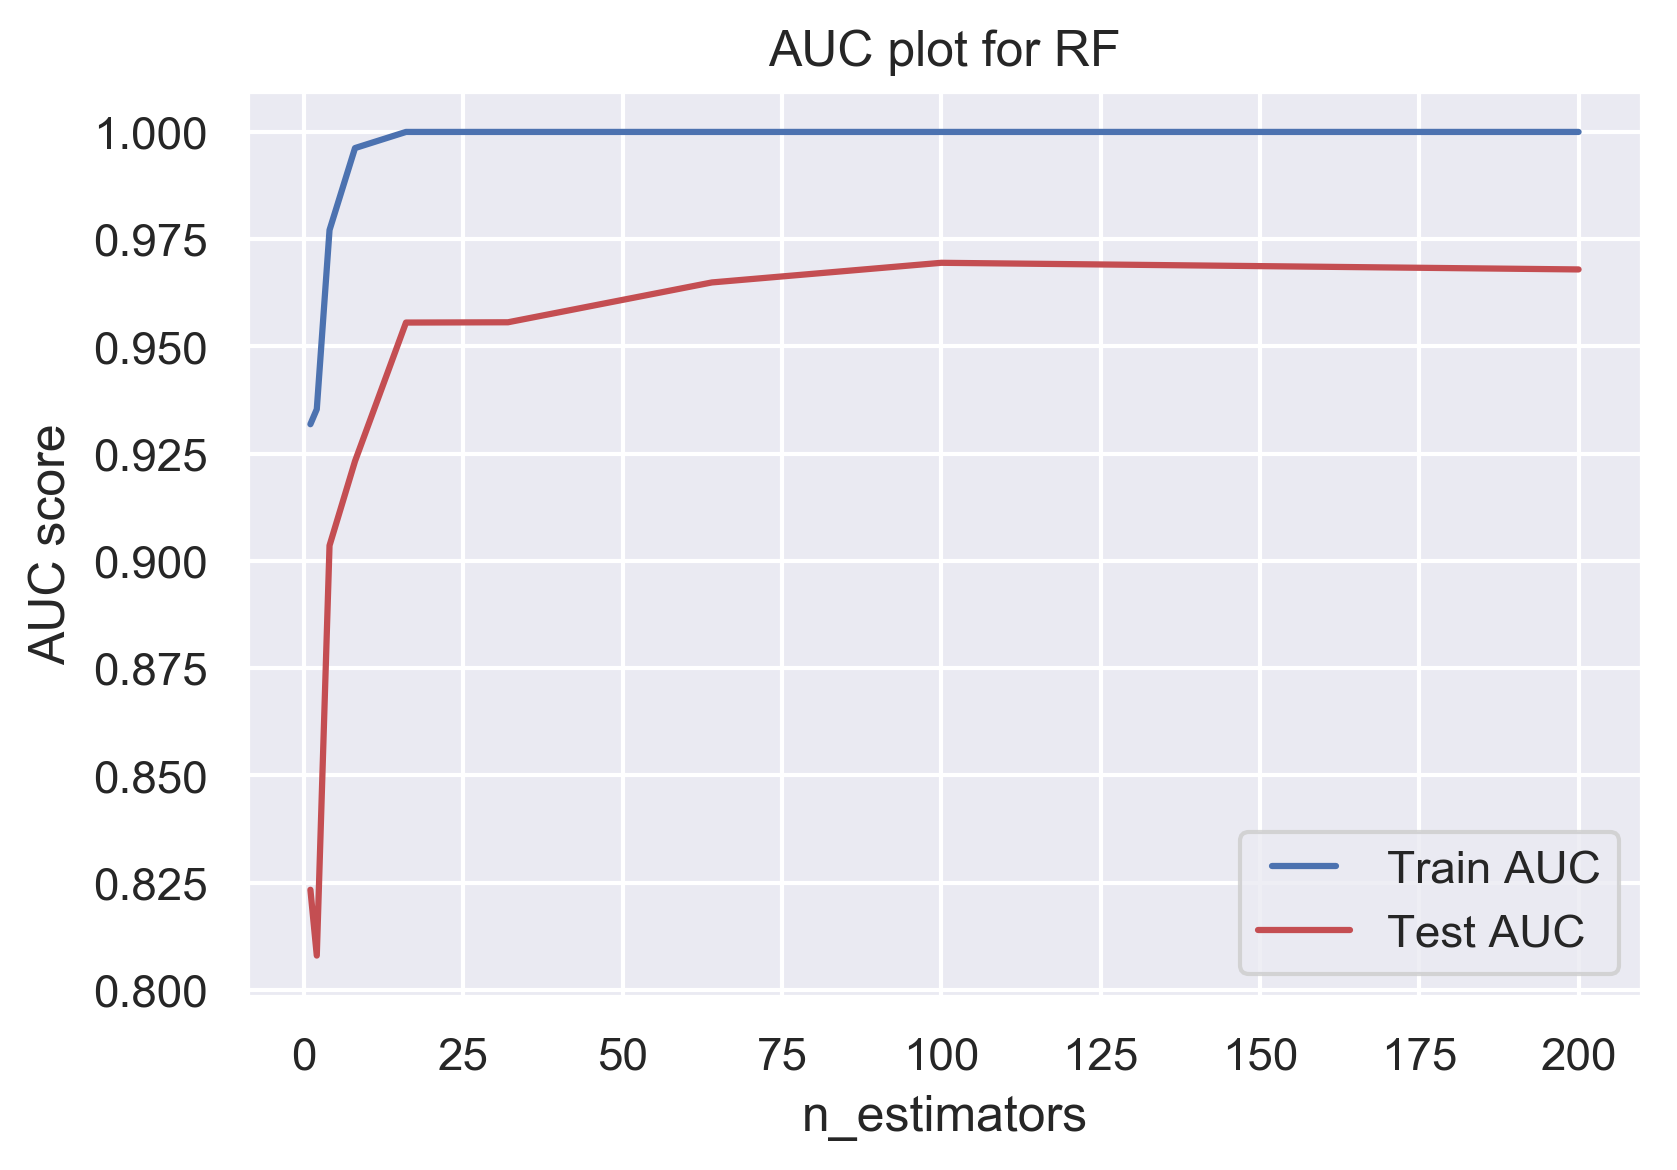
\includegraphics[width=6.1in]{assignment2/2-3-b-rf(n_estimator).png}
\caption{\label{fig:rfnest} Random Forest linear search for optimal n\_estimator parameter value}
\end{figure}

\clearpage{}
Next, a linear search was done to find the optimal value of tree depth. Figure~\ref{fig:rfnest} below shows the plot of AUC vs tree depth. We can see that the test and train data begin to diverge around a tree depth of 5, however test accuracy increases slightly until tree dept is 13. We decided to use a tree depth of 13 for the hyper parameter value.

\begin{figure}[!ht]
 \centering
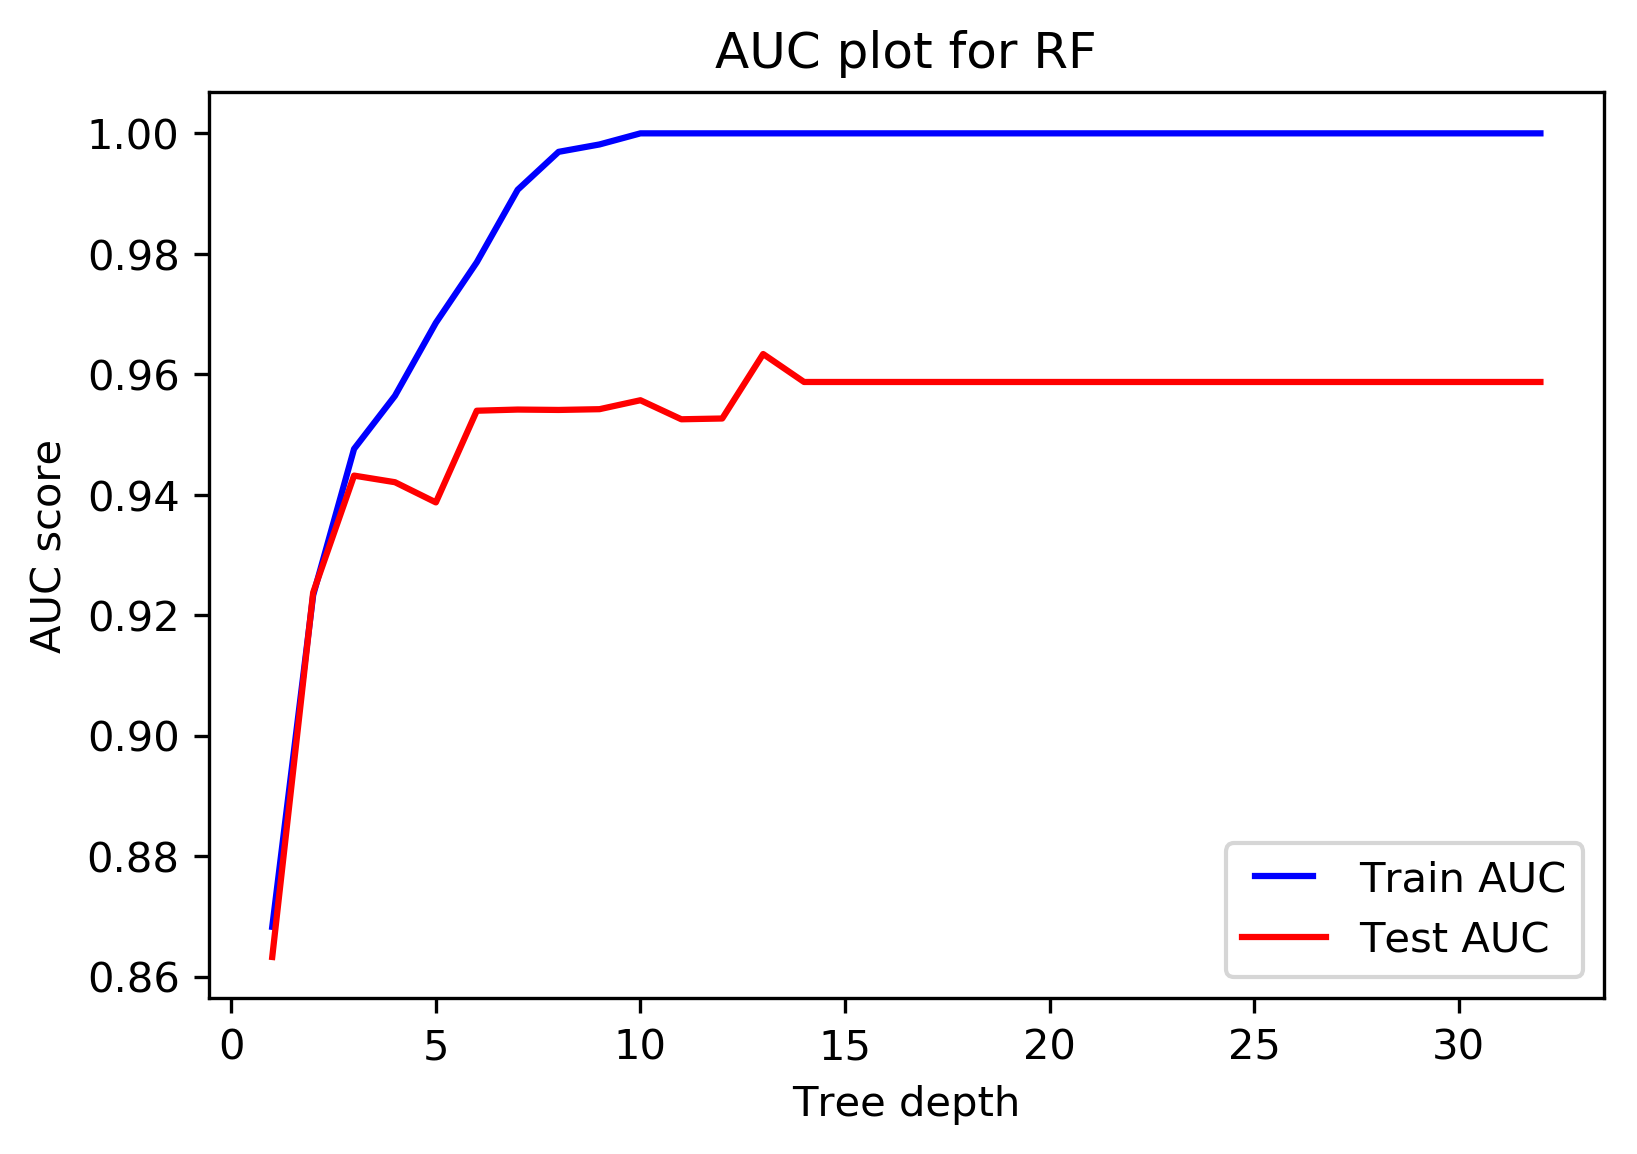
\includegraphics[width=6.1in]{assignment2/2-3-b-rf(Treedepth).png}
\caption{\label{fig:rftreedepth} Random Forest linear search for optimal treedepth parameter value}
\end{figure}

The result of the before and after for the random forest hyper parameter tuning can be seen in Figure~\ref{fig:resulstsrftune}. There was a fairly decent performance improvement from 0.95 f1 score to 0.97. Other methods to further improve performance could be explored such as grid search over a larger parameter space or boosting the tree by applying penalties to the cost function if complexity of the tree increases (also called regularization term).

\begin{figure}[!ht]
 \centering
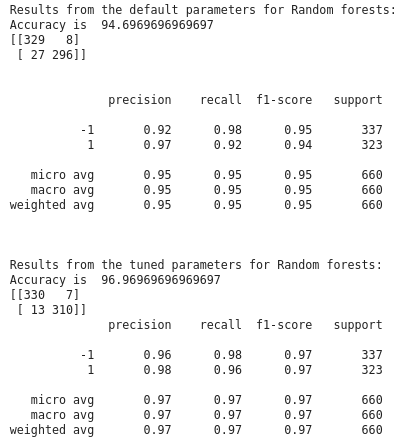
\includegraphics[height=3.5in]{assignment2/2-3-b-rfresult.png}
\caption{\label{fig:resulstsrftune} Performance Result for Random Forest before and after tuning hyper parameters}
\end{figure}

\clearpage{}
A similar process was done for the neural network model. We used a grid search to search over multiple parameters for the neural network model, this includes: hidden layer architecture, activation, solver, alpha, and batch size. We evaluated 4 architectures when training the neural network: (57,57,57), (57,57),(57,30,10), and (57,57,30,20,5). After performing the grid search it was determined that the best performing architecture was a 2 hidden layer with 57 neurons. The remaining parameters were as follows: "'activation': 'relu', 'alpha': 0.05, 'batch\_size': 70, 'hidden\_layer\_sizes': (57, 57), 'max\_iter': 2000, 'random\_state': 42, 'solver': 'adam'"

Figure~\ref{fig:resulstsnntune} below shows the result of the hyper parameter tuning. We can see that the neural network performance increased slightly from 0.90 to 0.92 f1 score. Due to limitation with sklearn library it was difficult to plot the training error and test error vs epoch using the MLPclassifier class. In the future keras will be used to better determine training metrics and characteristics when training. 

\begin{figure}[!ht]
 \centering
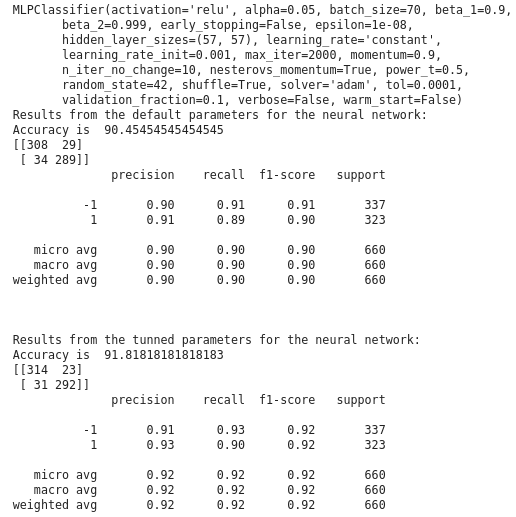
\includegraphics[height=3.5in]{assignment2/2-3-b-nnresult.png}
\caption{\label{fig:resulstsnntune} Performance Result for Neural Network before and after tuning hyper parameters}
\end{figure}




\subsubsection{Repeat each classification method 20 times by varying the split of the training-test set as in question 2-2. Report the average and standard deviation of classification performance on the test set regarding: accuracy, precision, recall, and F- Measure. Also report the training time and classification time of all the methods. Explain why the classification was repeated 20 times}

Each classification method was repeated 20 times for each value of k in \{4,5,6,7\}. The value K represented the fold in the cross validation. After completion the mean and standard deviation is calculated for each performance metric for every fold. Figures~\ref{fig:run1} to \ref{fig:run6} below show each table of values for each of the 6 classification methods.


\begin{figure}[!ht]
 \centering
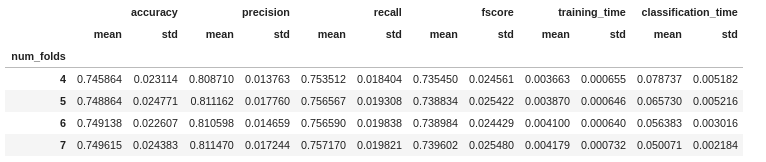
\includegraphics[width=\textwidth]{assignment2/2-4-run1.png}
\caption{\label{fig:run1} KNN performance metrics over 20 iterations of cross validation for different k folds}
\end{figure}

\begin{figure}[!ht]
 \centering
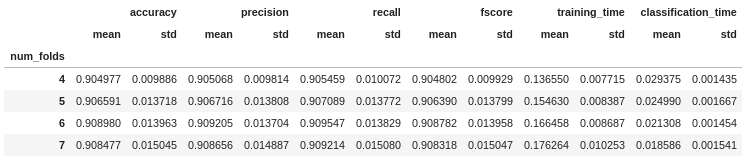
\includegraphics[width=\textwidth]{assignment2/2-4-run2.png}
\caption{\label{fig:run2} SVM performance metrics over 20 iterations of cross validation for different k folds}
\end{figure}

\begin{figure}[!ht]
 \centering
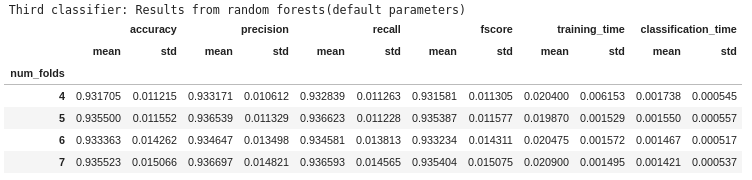
\includegraphics[width=\textwidth]{assignment2/2-4-run3.png}
\caption{\label{fig:run3} Random Forest with default parameters performance metrics over 20 iterations of cross validation for different k folds}
\end{figure}

\begin{figure}[!ht]
 \centering
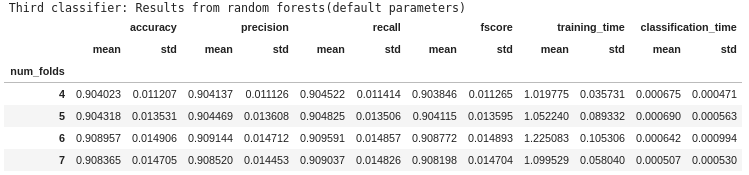
\includegraphics[width=\textwidth]{assignment2/2-4-run4.png}
\caption{\label{fig:run4} Neural Network with default parameters performance metrics over 20 iterations of cross validation for different k folds}
\end{figure}

\begin{figure}[!ht]
 \centering
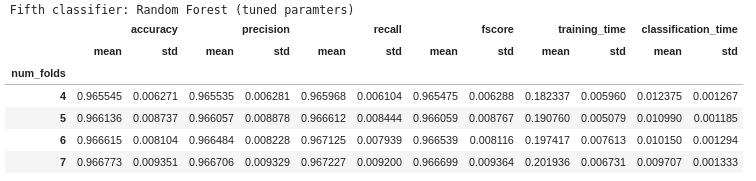
\includegraphics[width=\textwidth]{assignment2/2-4-run5.png}
\caption{\label{fig:run5} Random Forest with tuned parameters performance metrics over 20 iterations of cross validation for different k folds}
\end{figure}

\begin{figure}[!ht]
 \centering
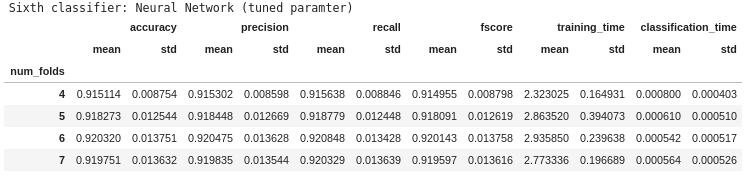
\includegraphics[width=\textwidth]{assignment2/2-4-run6.png}
\caption{\label{fig:run6} Neural Network with tuned parameters performance metrics over 20 iterations of cross validation for different k folds}
\end{figure}

\clearpage{}
Classification was repeated 20 times for the 6 models to get accurate measurements of the performance metrics recorded. The execution times for the algorithms can vary quite a bit depending on the system cpu usage and resources. Multiple threads running on the machine may take cpu clock cycles and delay algorithms from finishing the queued jobs. This is validated by the data collected. The standard deviation for the training time metric is the highest of all the recorded metrics. This is consistent with all algorithms.

\subsection{Obtained Results}

Based on the results obtained above, we see that k-NN performed the worst overall in terms of accuracy, precision, recall and f measure, however, it was the fastest in terms of training the model. Random forest with the tuned parameters performed the best among all, however, slower compared to Neural networks in terms of classification time. 

Neural networks in the other hand is the fastest at classifying but the slowest in training the model. SVM provided good metrics measurements compared to kNN but it took much more time to train the model and to classify. The tuned parameters for random forests and neural network performed significantly compared to their default hyper parameters. From this assignment, we can conclude that the Neural network and random forest are by far the best models for this type of data set when they are tuned. 

The information collected could be useful in determining which method to use for a similar data set in the future. First of all the performance of the models could be used to determine if the the model selected will meet the required accuracy for the application. training time and classification time are useful metrics to determine if the model selected will train or converge with the given resources or if predictions will be made quick enough (for example, real-time applications). Since our data set was fairly balanced the tables do not indicate which methods handle data imbalances better than others, however if these benchmarks were run once again with an imbalanced set more conclusions could be made.



\subsection{Feature Removal}
We can remove the redundant feature from the data set, Attributes that are not necessary decrease training speed,also tend to decrease our model's performance, most importantly,also generalization on the the test's performance is reduced.
I think with no prior domain knowledge about the data set and information we might have about the relationships between features, classification on two dimensions might result in a biased model. A brute force approach could be taken to systematically remove one feature at a time to determine feature importances for different models. 
\section{Part III: Nonlinear Dimensionality Reduction (for dataset B)}
\subsection{Apply LLE to the images of digit '3' only}

\subsection{Applying LLE to the images of digit '3' only}


\subsection{Applying ISOMAP to the images of digit '3' only}



\subsection{Naive Bayes classifier}


\bibliographystyle{IEEEtran}
\bibliography{ref}


%
% ---- Bibliography ----
%
\bibliographystyle{splncs04}
\begin{thebibliography}{8}

\bibitem{ref_article1}
Macek, K. "Pareto principle in datamining: an above-average fencing algorithm." Acta Polytechnica 48.6 (2008).


\bibitem{ref_url1}
  \url{https://scikit-learn.org/stable/modules/generated/sklearn.tree.DecisionTreeClassifier.html}.
  
\bibitem{ref_url2}
  \url{https://elitedatascience.com/imbalanced-classes}. 
  
\bibitem{ref_url3}
  \url{https://scikit-learn.org/stable/modules/tree.html#tree-algorithms}. 
\end{thebibliography}
% ------------------------------------------------------------------------------
% End document
% ------------------------------------------------------------------------------
\end{document}